\chapter{Overview}

\numberwithin{equation}{chapter}

\section{Problem statement}
Size of database/dictionary
Quality

In order to find 
1. coding signals 
2. find a good dictionary

analog problem video compression but with less corelation between images and still image 

\subsection{criteria}
Convergence of the dictionary learning
Quality increase with size increase 

\subsection{dictionaries for signal representation}
Dictionaries is a collection of ordered elements with an index.
Atom is am small unit of something big.
The Cambridge Advanced Learner defines a code as ``..a system of numbers, letters or signals which is used to represent something in a shorter or more convenient form''
A sparse code is a sparse vector of coefficents that is used to linear combie a small selection of atoms from a dictionarie.
As a matter of fact a good dictionary is essential for a good signal approximation. \cite{} Finding this dictionarie has become a major task/problem in the last 15 years.

\section{signal representation/analysis}
Signal transforms \cite{sparse intro} that far back in the early 60s.
FFT in 65s

approximate signals via combination of limited signal samples
Why?
signal analysis, compression, de-noise etc.

The early approaches in the 60s used combinations of cosine transformations. Coming from a continues representation this makes 
actually sense. The signal could be represented via ....

In 80s the search for better transformation basis became a major role in signal representation. \cite{}

\subsection{discrete signals}
Rather then using continues signal we concentrate on discrete signal representation.
Continues signals would be better for .... . But our signal (image etc.) will be discrete anyway becaus of their initial digital representation. 
Besides the problem of coding becomes different in the continues space \cite{} Because of ...

\subsection{splitting the problem}
\cite{Rubinstein2010}
In the last 15 years 

the idea came up to interpret the basis transforms as sparse linear combination of dictionary atoms.
see \cite{Olshausen1997} and \cite{}
The benefit from this approach/direction was that you could decouple signal coding and dictionary design.
Separating the problem into two distinct problems made the search for task specific and .... more flexible \cite{?}.

Two separate tasks.
Coding the signal. Design of the dictionary.

\subsection{dictionaries and application}
Signal representation via linear combination of few signal vectors from a dictionary.
Benefits of dictionaries


\section{sparse codes/coding}
Consider $X$ as matrix with $n$ columns each column $x_{i}$ representing a signal described by a single vector of signal length $m$.
The dictionary $D$ is another matrix with $p$ columns where each column reprensents an atom signal with the same dimension and size as a single signal $x_{i}$ from $X$.
The sparse vector $\alpha$ is linear combination of a few non orthonormal atoms from D that is close to the signal X.
try to keep coefficient vector sparse
Sparse coding is the 
\[
\underbrace{\begin{pmatrix} x_1 \\ x_2 \\ \vdots \\ x_n \end{pmatrix}}_{signal} \approx \underbrace{\begin{pmatrix} d_1  d_2 \cdots d_n \end{pmatrix}}_{\textrm{dictionary atoms}}
\underbrace{\begin{pmatrix} \alpha_1 \\ \alpha_2 \\ \vdots \\ \alpha_n \end{pmatrix}}_{\textrm{keep sparse}}
\]
solve under-determined linear system
we want the sparsest solution
\begin{align}
\min_{\alpha\in\mathbb{R}^{p}}  \lVert x - D\alpha \rVert^{2}_{2} + \underbrace{\psi(\alpha)}_{regularization}
\end{align}
measure sparsity via       l0-norm       $\lVert\alpha\rVert_{0}$

\begin{figure}
\centering
%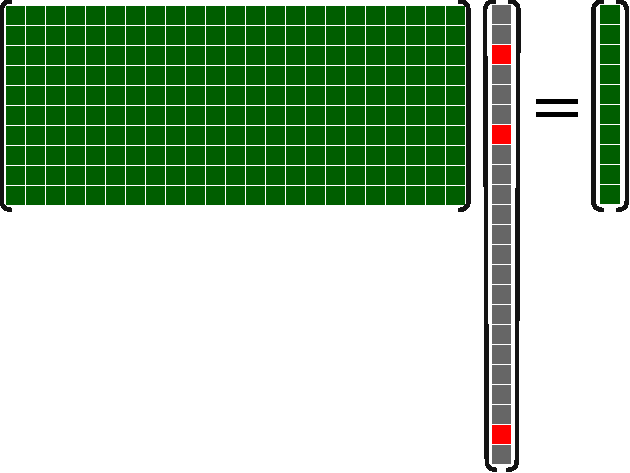
\includegraphics[width = 0.66\textwidth]{images/Da_x.pdf} % Or .pdf
\caption{Sparse Coding}
\label{fig:da_x}
\end{figure}


In the last 15 years several sparse coding algorithms have been proposed. 
Some that solve the initial problem <> greedyly, the (orthogonal) matching pursuit, and others which modified the problem to become convex/linear. These primary derive from the numerical domain in the form of 
large linear system solvers with few optimization constraints. The LARS-Lasso, basis pursuit, FOCUSS?


$\lVert\alpha\rVert_{0}$ makes the problem NP-hard
to get best solution you need to test every combination
Solution:
use greedy approach or make problem convex (e.g. use $\lVert\alpha\rVert_{1}$)
the most common algorithms are the following ones.


\subsection{matching pursuit}
The algorithm calculates a coefficient vector $\alpha$ which is an approximate solution of the following NP-hard problem
\begin{align}
\min_{\alpha\in\mathbb{R}^{p}}  \lVert x - D\alpha \rVert^{2}_{2} \textrm{ s.t. } \lVert \alpha \rVert_{0} \leq L
\end{align}
or
\begin{align}
\min_{\alpha\in\mathbb{R}^{p}}   \lVert \alpha \rVert_{0}   \textrm{ s.t. } \lVert x - D\alpha \rVert^{2}_{2} \leq \epsilon
\end{align}
\cite{Mallat1993}
\begin{algorithm}
\begin{algorithmic}
\STATE i=0
\end{algorithmic}
\end{algorithm}

\subsection{orthogonal matching pursuit}
\cite{Pati1993}
\label{sec:omp}
\begin{algorithm}
\begin{algorithmic}
\STATE i=0
\end{algorithmic}
\end{algorithm}

\subsection{LARS-Lasso}
The LASSO (least absolute shrinkage and selection operator) is a regularized version of a least squares solution.
The regularized version is found by adding a constraint that induces the $L_1$-norm of the solution to be small.
There are several ways to compute the LASSO. .. ...... \cite{} 
The LARS algorithm ... \cite{Efron2004}
The LARS-Lasso is a algorithm to solve the LASSO with the help of least angle regression
as described in \cite{Efron2004}. It is a modified version of the LARS where ....



\begin{align}
\min_{\alpha\in\mathbb{R}^{p}}  \lVert x - D\alpha \rVert^{2}_{2} \textrm{ s.t. } \lVert \alpha \rVert_{1} \leq L
\end{align}
or
\begin{align}
\min_{\alpha\in\mathbb{R}^{p}}   \lVert \alpha \rVert_{1}   \textrm{ s.t. } \lVert x - D\alpha \rVert^{2}_{2} \leq \epsilon
\end{align}

\begin{algorithm}
\begin{algorithmic}
\STATE i=0
\end{algorithmic}
\end{algorithm}

Some limitations of the LARS-Lasso
\begin{description}
 \item[todo] \Todo 1/2/3 see online
\end{description}


\subsection{usage/application}
\begin{description}
\item[noise reduction]
Remove noise from a signal. Using the fact that sparse coding 
is an approximation of signal that looses .... in its encoding process. 
\cite{Elad2006}

\item[inpainting]
fill missing parts by removing rows from the dictionary
Train with the original image
\cite{mairal08sparse}

\item[compression] An example for this is the compression of facial images by Bryt and Elad \cite{Bryt2008}.
\item[classification] Examples for this can be found in \cite{Mairal2008b} and \cite{Bar2009}.
\end{description}



\section{Dictionaries/representation data}
\subsection{analytical}
\begin{description}
 \item[cosine]
 \item[wavelets]
 \item[curvelets/contourlets/bandelets]
\end{description}

\subsection{learned over-complete}
recent research has shown that learnd dictionaries show better compression quality than small analytic dictionaries \cite{Aharon2006} \cite{Chen1998} 


In the last decade several learning algorithms have been proposed which try to a universal basis that 
can sparsly reconstruct a set of "trainig data" with minimal error. 
K-SVD
MOD
Online learning
Mairal2010

\subsubsection{k-svd}
\subsubsection{online learning}
Mairal .... \cite{Mairal2010}

\section{Learning for the Task}
It has been shown that learning basis specialy for certain tasks can lead to the best results\cite{}.  <>
Based on this discovery we will concentrate on a specific class. <> Join the basis for natural images and cartoon/line images.
We will also concentrate on real practical data. This means typically 3-channel data of 1+ megapixels images found on image hosting services like flickr, twitpic, etc.

Current research is primary concentrating on other tasks. 
Like ... related work :)

\subsection{improvements}

\begin{description}
\item[multi-scale]
Rather than encoding uniform segments of a bigger signal this technique encodes different sized 
segments (multiple times of the default segment). The idea is that aligned smooth regions with low variance can be 
can be combined an encoded as one signal rather than e.g. 4. \cite{saprio}

\item[multi-channel]
coding every channel separate or combine them
into single signal. can lead to color bleeding \cite{mairal08sparse}
fortunately this problem vanishes with big dictionaries and large training sets. \cite{mairal08sparse}

\item[double sparsity]
Rather then directly using a collection of basis/atom signals as a dictionary. This approach uses sparse coding
to encode the signals of a bigger dictionary with the help of a smaller on. \cite{double sparsity}

\item[group sparsity]
similar patches should admit similar patterns
\cite{double sparsity}

\item[hirarchy/structure]
Adding hirarchy/structure to dictionaries can lead to faster coding or use in structure analysis ( text documents )
\cite{Jenatton2010}

\end{description}




\section{Related work}
\begin{description}
\item[compression of facial images] In 2008 Bryt and Elad \cite{Bryt2008} 
\item[training with a neural network]
Learning Multiple Layers of Features from Tiny Images \cite{Krizhevsky2009}
\item[noise reduction]
\item[in-painting]
\end{description}



\section{goal of this thesis}
Evaluate the quality and size of learned big redundant dictionaries for 
optimal sparse coding of large image databases.

Observation of problems (encoding time, quality benefit, etc.)

Search for a universal dictionary for combination natural and artificial images
 
Convergence of different sizes and configurations of learned dictionaries.
how many elements for a 'good' sparse representation?

\Todo{OPTIONAL add structure for speed and model improvements Multi-scale, multi-channel, hierarchy}


Improve compression vs. jpeg/jepg2000 and possible usage as an image descriptor.
